%%%%%%%%%%%%%%%%%%%%%%%%%%%%%%%%%%%%%%%%%%%%%%%%%%%%%%%%%%%%%%%%%%%%%%%%
%    INSTITUTE OF PHYSICS PUBLISHING                                   %
%                                                                      %
%   `Preparing an article for publication in an Institute of Physics   %
%    Publishing journal using LaTeX'                                   %
%                                                                      %
%    LaTeX source code `ioplau2e.tex' used to generate `author         %
%    guidelines', the documentation explaining and demonstrating use   %
%    of the Institute of Physics Publishing LaTeX preprint files       %
%    `iopart.cls, iopart12.clo and iopart10.clo'.                      %
%                                                                      %
%    `ioplau2e.tex' itself uses LaTeX with `iopart.cls'                %
%                                                                      %
%%%%%%%%%%%%%%%%%%%%%%%%%%%%%%%%%%
%
%
% First we have a character check
%
% ! exclamation mark    " double quote  
% # hash                ` opening quote (grave)
% & ampersand           ' closing quote (acute)
% $ dollar              % percent       
% ( open parenthesis    ) close paren.  
% - hyphen              = equals sign
% | vertical bar        ~ tilde         
% @ at sign             _ underscore
% { open curly brace    } close curly   
% [ open square         ] close square bracket
% + plus sign           ; semi-colon    
% * asterisk            : colon
% < open angle bracket  > close angle   
% , comma               . full stop
% ? question mark       / forward slash 
% \ backslash           ^ circumflex
%
% ABCDEFGHIJKLMNOPQRSTUVWXYZ 
% abcdefghijklmnopqrstuvwxyz 
% 1234567890
%
%%%%%%%%%%%%%%%%%%%%%%%%%%%%%%%%%%%%%%%%%%%%%%%%%%%%%%%%%%%%%%%%%%%
%
\documentclass[12pt]{article}
\usepackage{biblatex}
\usepackage{xcolor}
\usepackage{amsmath}
\usepackage{authblk}
\usepackage{graphicx}
\addbibresource{biblio.bib}
\begin{document}

\title{Optimization of stellarator access ports for maintenance}

\author[1]{A. Baillod}
\author[1]{E. J. Paul}
\affil[1]{Department of Applied Physics and Applied Mathematics, Columbia University, New York, New York 10027, USA}
\date{\today}                     %% if you don't need date to appear
\renewcommand\Affilfont{\itshape\small}
\maketitle


\begin{abstract}
\begin{itemize}
	\item MAIS SALUT DIT VOIR
\item Future magnetic confinement fusion power plant will require remote maintenance to replace the breeding blanket
\item Stellarators have a complex geometry that can be optimized for better accessibility
\item In this paper, we describe how the maximum port size can be evaluated given a vessel and the coils geometry
\item We show that the port size can be optimized to allow better access to the in-vessel components while keeping the same magnetic field quality
\item Three standard stellarators are considered, namely a quasi-axisymmetric, a quasi-helically symmetric and a quasi-isodynamic configuration
\item ...
\end{itemize}
\end{abstract}


\section{Introduction}

Core motivation papers are:
\begin{itemize}
    \item Paper by Bachmann \textit{et.al.} \cite{bachmann_2022} on DEMO remote maintenance system design
    \item ARIES-CS design paper \cite{raffray_2008} by A. R. Raffray \textit{et.al.}
    \item Private communication with L. Jorrit
\end{itemize}

Main points are
\begin{itemize}
    \item During the lifetime of a reactor, the breeding blanket (BB) will need to be replaced {\color{red}source?}
    \item This maintenance process will have to be done remotely using remote handling (RH) tools
    \item The complexity of the operation and reactor down-time increases with the number of elements to be replaced
    \item The number of elements is set by their size, which in turn is set by the size of the port used to access the in-vessel components
    \item Overall, large ports are desirable
\end{itemize}

Paper contribution
\begin{itemize}
    \item Development of a new method to measure the maximum port size
    \item Application to three different configuration 
    \item Optimization to show that the port size can be increased
    \item Comparison between QA, QI and QH access?
\end{itemize}

Paper is organized as follows
\begin{itemize}
    \item In section \ref{sec.metric} we describe how the port size is evaluated given a vessel boundary and the geometry of the coils
\end{itemize}


\section{Port size evaluation} \label{sec.metric}
We describe in this section how the port size is evaluated for any given point $\mathbf{\tilde x}$ on the vessel boundary $\delta V$ --- here we assume that the surface $\delta V$ encloses a toroidal volume $\mathcal{V}$, which contains the plasma and blanket, and that the coils are outside $\mathcal{V}$. The idea is to project the vessel boundary and the coils on a plane tangent to the vessel boundary at $\tilde{\mathbf{x}}$. The maximum circular port is then the largest circle centered at $\tilde{\mathbf{x}}$ that fits within the vessel projection and does not intersect any of the projected coils. Not all segments of the coils are of interest though; only segment "in front" of the vessel (this concept will be defined in more details below) have to be taken into account. We will use three different coordinate systems; the first one is the cartesian coordinate system $(\hat{\mathbf{i}},\hat{\mathbf{j}},\hat{\mathbf{k}})$, in which the coils, represented as filaments, will be expressed. The second coordinate system is the standard cylindrical coordinate system $(\hat{\mathbf{r}},\hat{\mathbf{\phi}},\hat{\mathbf{k}})$, which defines the toroidal angle $\phi$, and will be used to represent the vessel boundary $\delta\mathcal{V}$. Finally, to evaluate which segment of which coil might get in the way of the access path, we will need a third coordinate system, that we denote $(\hat{\mathbf{n}},\hat{\mathbf{t}},\hat{\textbf{b}})$ and is defined below.

We parametrize the vessel boundary $\delta \mathcal{V}$ by a double Fourier series, $\mathbf{x}^v(\theta,\phi)=R(\theta,\phi)\hat{\mathbf{r}}+Z(\theta,\phi)\hat{\mathbf{k}}\in\delta \mathcal{V}$ with 
\begin{align}
    R(\theta,\phi) &= \sum_{m=0}^{M}\sum_{n=-N}^N R_{mn}\cos(m\theta-nN_f\phi)\\
    Z(\theta,\phi) &= \sum_{m=0}^{M}\sum_{n=-N}^N Z_{mn}\sin(m\theta-nN_f\phi),
\end{align}
where $\theta$ is a poloidal angle, $(M,N)$ are the largest poloidal and toroidal Fourier mode number respectively, $(R_{mn},Z_{mn})$ are the Fourier coefficients for the coordinate $R$ and $Z$ respectively, $N_f$ is the number of field period (discrete toroidal symmetry) of the boundary, and stellarator symmetry \cite{dewar_1998} is assumed. We discretize the vessel boundary with a uniform grid in the poloidal and toroidal direction, $\mathbf{x}^v_{i} = \mathbf{x}^v(\theta_i,\phi_i)$, with $i\in\{1,\ldots, N_\theta N_\phi\}$.


\begin{figure}
    \centering
    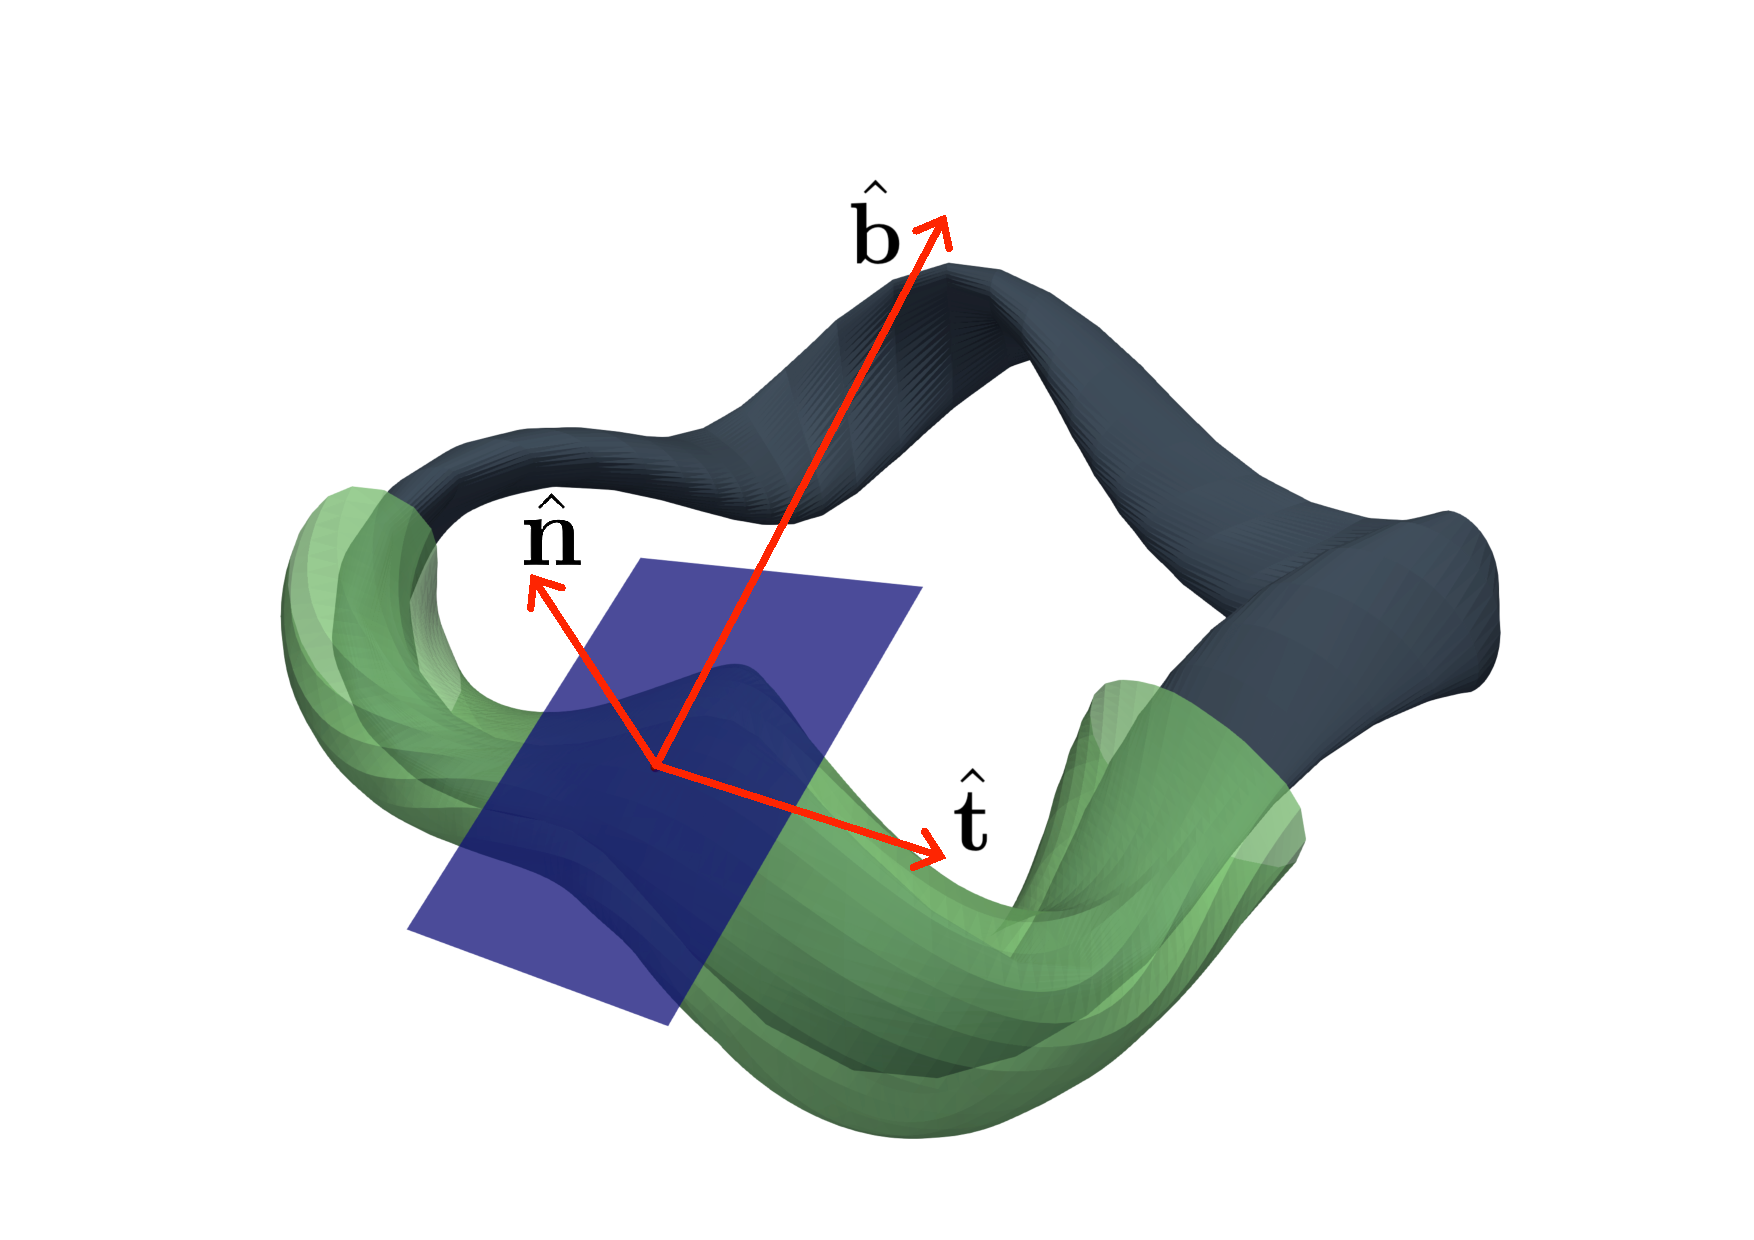
\includegraphics[width=.75\textwidth]{figures/tangent_plane_coordinate.pdf}\\
    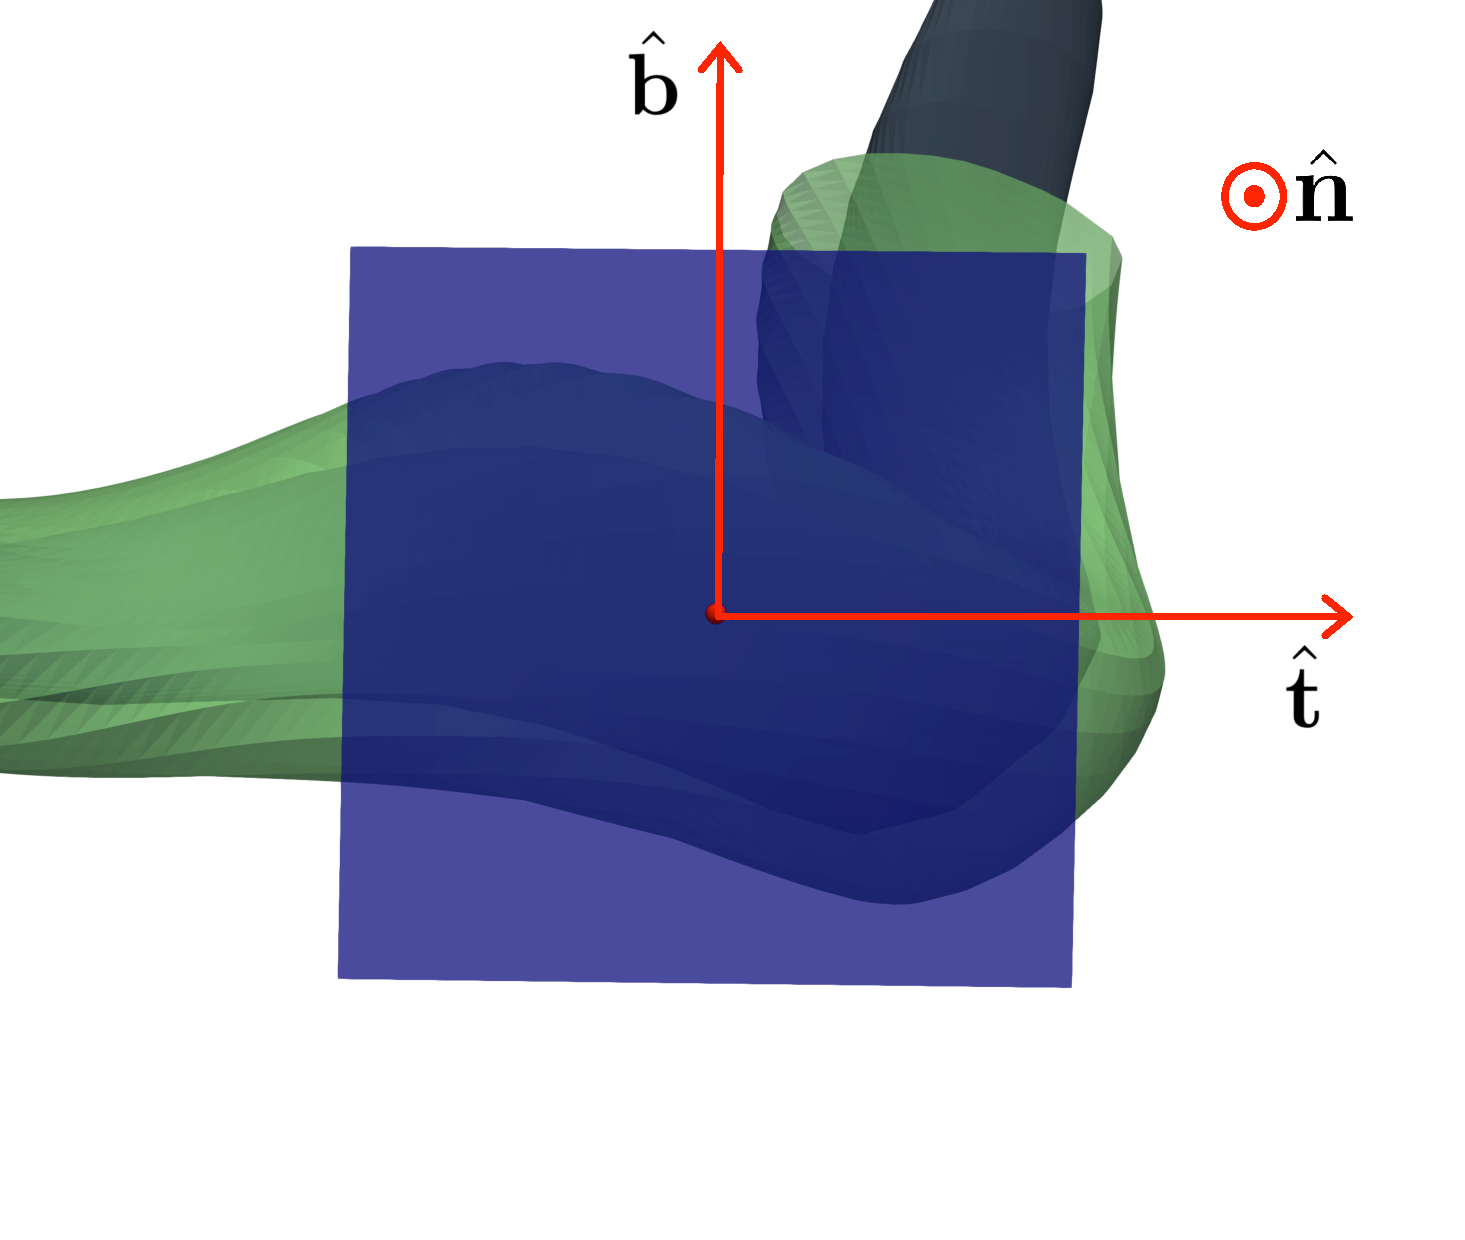
\includegraphics[width=.75\textwidth]{figures/tangent_plane_coordinate_front.pdf}
    \caption{Sketch of the $(\hat{\mathbf{n}},\hat{\mathbf{t}},\hat{\textbf{b}})$ coordinate system. Black toroidal surface: plasma boundary. Green surface: three-halves field period of the vessel boundary $\delta\mathcal{V}$. Blue plane: plane tangent to $\delta\mathcal{V}$ at $\tilde{\mathbf{x}}\in\delta\mathcal{V}$. Top: side view, bottom: front view.}
    \label{fig.tangent_coordinates}
\end{figure}

Given a point $\mathbf{\tilde x}=\mathbf{x}^v(\tilde{\theta},\tilde{\phi})$ on $\mathcal{S}$, we construct the coordinate system $(\hat{\mathbf{n}},\hat{\mathbf{t}},\hat{\textbf{b}})$, with $\mathbf{\tilde x}$ as origin, and where $\hat{\mathbf{n}}$ is a unitary vector normal to $\mathcal{S}$ at $\mathbf{\tilde x}$, pointing outwards from $\mathcal{V}$, $\hat{\mathbf{t}}$ is a unitary vector tangential to the vessel boundary at $\mathbf{\tilde x}$ and pointing in the direction of $\partial \mathbf{\tilde x}/\partial \phi$, and $\hat{\mathbf{b}}=\hat{\mathbf{n}}\times\hat{\mathbf{t}}$ (see Figure \ref{fig.tangent_coordinates}). This coordinate system is nothing else than a rotated and translated cartesian coordinate system, and the coordinates of any point $\mathbf{x}=x_n\hat{\mathbf{n}}+x_t\hat{\mathbf{t}}+x_b\hat{\textbf{b}}$ are easily obtained by solving the linear system
\begin{equation}
\mathbf{M}(\tilde{\mathbf{x}})\left(\begin{matrix}
    x_n\\
    x_t\\
    x_b
\end{matrix}\right) = \mathbf{x}-\mathbf{\tilde x},\label{eq.projection}
\end{equation}
where $\mathbf{M}$ is a $3\times 3$ matrix with columns set by the vectors $(\hat{\mathbf{n}},\hat{\mathbf{t}},\hat{\textbf{b}})$ written in cartesian coordinates. Once projected on the $(\hat{\mathbf{t}},\hat{\mathbf{b}})$-plane, the vessel boundary $\delta\mathcal{V}$ is bounded by two curves, that we call the upper envelop $\mathbf{u}(x)$ and lower envelop $\mathbf{l}(x)$. Writing 
\begin{align}
    x_b(\theta,\phi) &= \left[\mathbf{M}^{-1}(\mathbf{x}^v(\theta,\phi)-\tilde{\mathbf{x}})\right]\cdot \hat{\mathbf{b}}\\
    x_t(\theta,\phi) &= \left[\mathbf{M}^{-1}(\mathbf{x}^v(\theta,\phi)-\tilde{\mathbf{x}})\right]\cdot \hat{\mathbf{t}},
\end{align}
we define
\begin{align}
    \mathbf{u}(x) &= u_n(x)\hat{\mathbf{n}} + x\hat{\mathbf{t}} + u_b(x)\hat{\mathbf{b}}\label{eq.u-def}\\
    u_b(x) &= \max_{\substack{(\theta,\phi) \in [0,2\pi]\times[0,2\pi/N_f]\\ u_t=\text{const}}} x_b(\theta,\phi),
\end{align}
where $u_n(x)$ is chosen such that $\mathbf{u}\in\partial\mathcal{V}$. Similarly,
\begin{align}
    \mathbf{l}(x) &= l_n(x)\hat{\mathbf{n}} + x\hat{\mathbf{t}} + l_b(x)\hat{\mathbf{b}}\\
    l_b(x) &= \min_{\substack{(\theta,\phi) \in [0,2\pi]\times[0,2\pi/N_f]\\ u_t=\text{const}}} x_b(\theta,\phi).\label{eq.l-def}
\end{align}
The curves $u_b(x)$ and $l_b(x)$ form the non-convex hull of the vessel boundary projected on the $(\hat{\mathbf{t}}, \hat{\mathbf{b}})$-plane (see Figure \ref{fig.non-convex-hull}), and are evaluated using the $\chi$-algorithm proposed by M. Duckham \textit{et.al.} \cite{duckham_2008}. The maximum port size around $\tilde{\mathbf{x}}$ is set by the minimal distance to the upper or lower envelop,
\begin{equation}
    r^{lim}_{port} = \min_{x}[\mathbf{u}(x)\cdot\hat{\mathbf{b}},\mathbf{l}(x)\cdot\hat{\mathbf{b}}]. \label{eq.max_port_size}
\end{equation}
Note that the maximum port size defined by Eq.(\ref{eq.max_port_size}) depends on the position of the port $\tilde{\mathbf{x}}$.

\begin{figure}
    \centering
    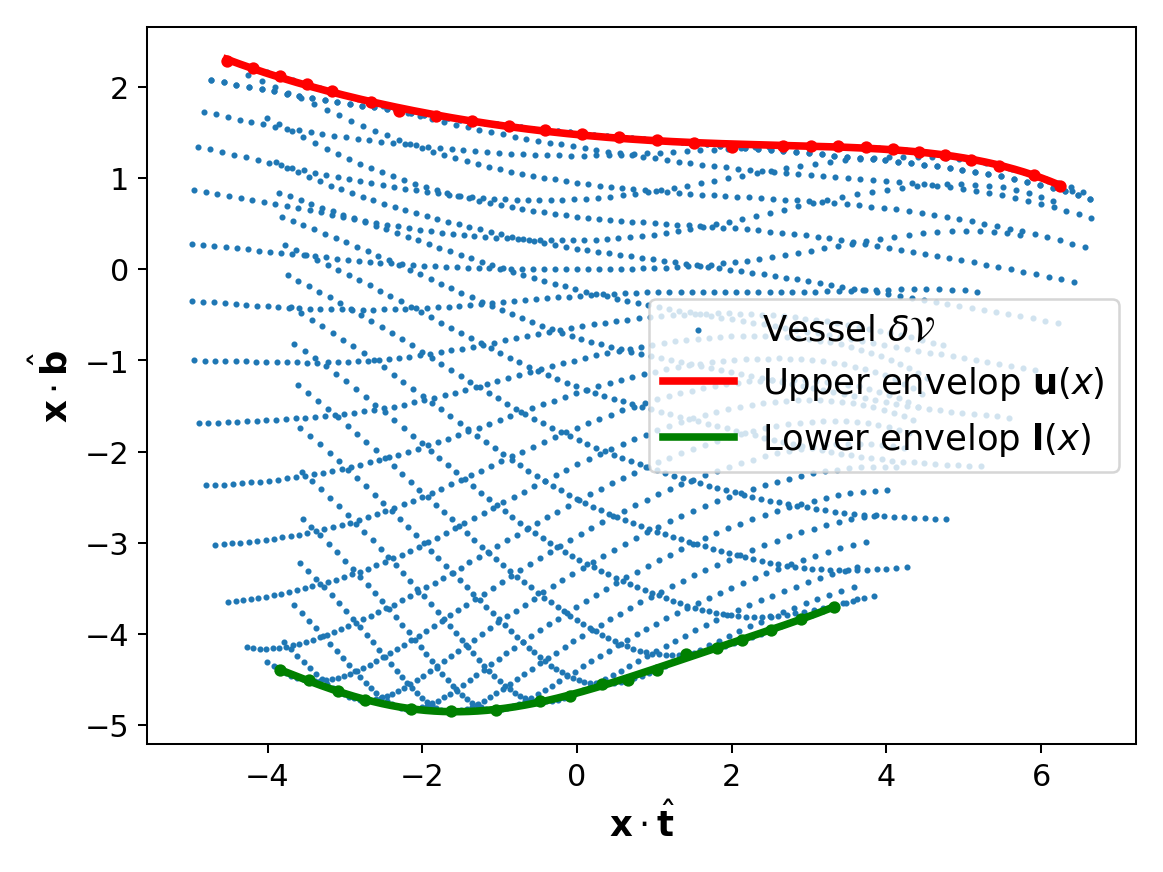
\includegraphics[width=.75\linewidth]{figures/envelop_vizualization.png}
    \caption{Vizualization of the upper and lower envelop, $\mathbf{u}(x)$ and $\mathbf{l}(x)$, as defined by Eqs.(\ref{eq.u-def})-(\ref{eq.l-def}).}
    \label{fig.non-convex-hull}
\end{figure}





%These curves are difficult to extract numerically --- this problem would require the implementation of a specific non-convex hull algorithm. Instead, for each toroidal plane $\phi=\text{const}$ reasonably close from $\tilde{\mathbf{x}}$, we find the points with maximum and minimum $\hat{b}$-coordinate. Fitting the $\hat{\mathbf{n}}$- and $\hat{\mathbf{b}}$-coordinate of the maxima and the minima with a 5$^{th}$-order polynomial leads to a reasonable approximation of $\mathbf{u}(x_t)$ and $\mathbf{l}(x_t)$ respectively. We then set the maximum port size around $\tilde{\mathbf{x}}$ as the minimal distance to the upper and lower envelops, $r^{max}_p = \min_{x_t}[\mathbf{u}(x_t)\cdot\hat{\mathbf{b}},\mathbf{l}(x_t)\cdot\hat{\mathbf{b}}]$.




We now consider $N_{coils}$ coils, that we represent by filaments $\Gamma_j$ (curve of zero width) in cartesian coordinates. We express their position as Fourier series as proposed by Zhu \textit{et.al.} \cite{zhu_2017}, $\mathbf{x}^c(l) = x^c(l)\hat{\mathbf{i}} + y^c(l)\hat{\mathbf{j}} + z^c(l)\hat{\mathbf{k}}$, where
\begin{align}
    x^c(l) &= x^c_{e,0} + \sum_{k=1}^{N_k} x^c_{e,1}\cos(2\pi kl) + \sum_{k=1}^{N_k} x^c_{o,1}\sin(2\pi kl)\\
    y^c(l) &= y^c_{e,0} + \sum_{k=1}^{N_k} y^c_{e,1}\cos(2\pi kl) + \sum_{k=1}^{N_k} y^c_{o,1}\sin(2\pi kl)\\
    z^c(l) &= z^c_{e,0} + \sum_{k=1}^{N_k} z^c_{e,1}\cos(2\pi kl) + \sum_{k=1}^{N_k} z^c_{o,1}\sin(2\pi kl),
\end{align}
with $l\in[0,1]$. Each coil filament is then discretized in $N_p$ quadrature points $(x^c_p,y^c_p,z^c_p)=(x^c(l_p),y^c(l_p),z^c(l_p))$, with $l_p=(p-1)/N_p$, $p\in\{1, \ldots, N_p\}$. We pack all coils quadrature points in a single array of size $N_{coils}N_p$, and denote by $\mathbf{x}^c_i$ their position. Again, solving Eq.(\ref{eq.projection}) provides the coils quadrature points coordinate in the $(\hat{\mathbf{n}},\hat{\mathbf{t}},\hat{\textbf{b}})$ coordinate system (see Figure \ref{fig.coil_projection}),
\begin{equation}
    \mathbf{x}^c_i = x^c_i\hat{\mathbf{i}} + y^c_i\hat{\mathbf{j}} + z^i_i\hat{\mathbf{k}} = n^c_{i}\hat{\mathbf{n}} + t^c_i\hat{\mathbf{t}} + b^c_i\hat{\mathbf{b}}.
\end{equation}
\begin{figure}
    \centering
    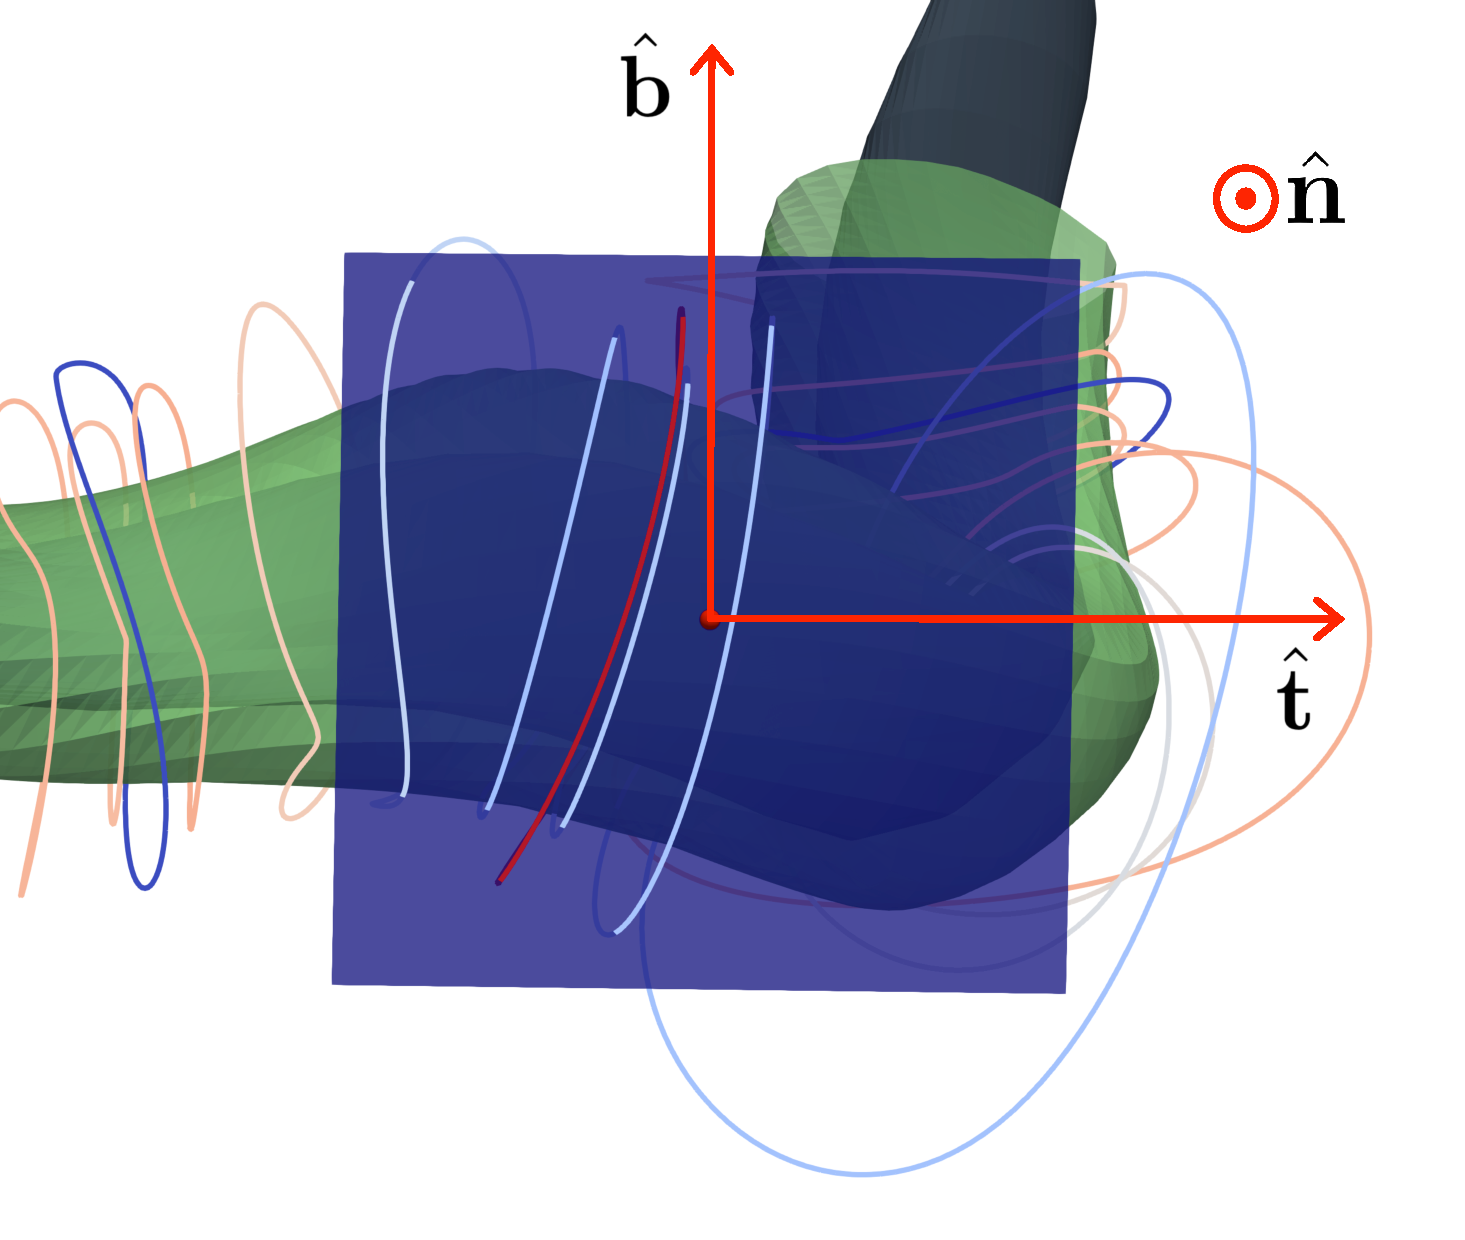
\includegraphics[width=\textwidth]{figures/tangent_plane_with_coils.pdf}
    \caption{Front view of the plasma surface, vessel and coils.}
    \label{fig.coil_projection}
\end{figure}
Now, we consider only coil elements standing in front of the vessel, \textit{i.e.} points that satisfy the following conditions (see Figure \ref{fig.sketch_condition}):
\begin{figure}
    \centering
    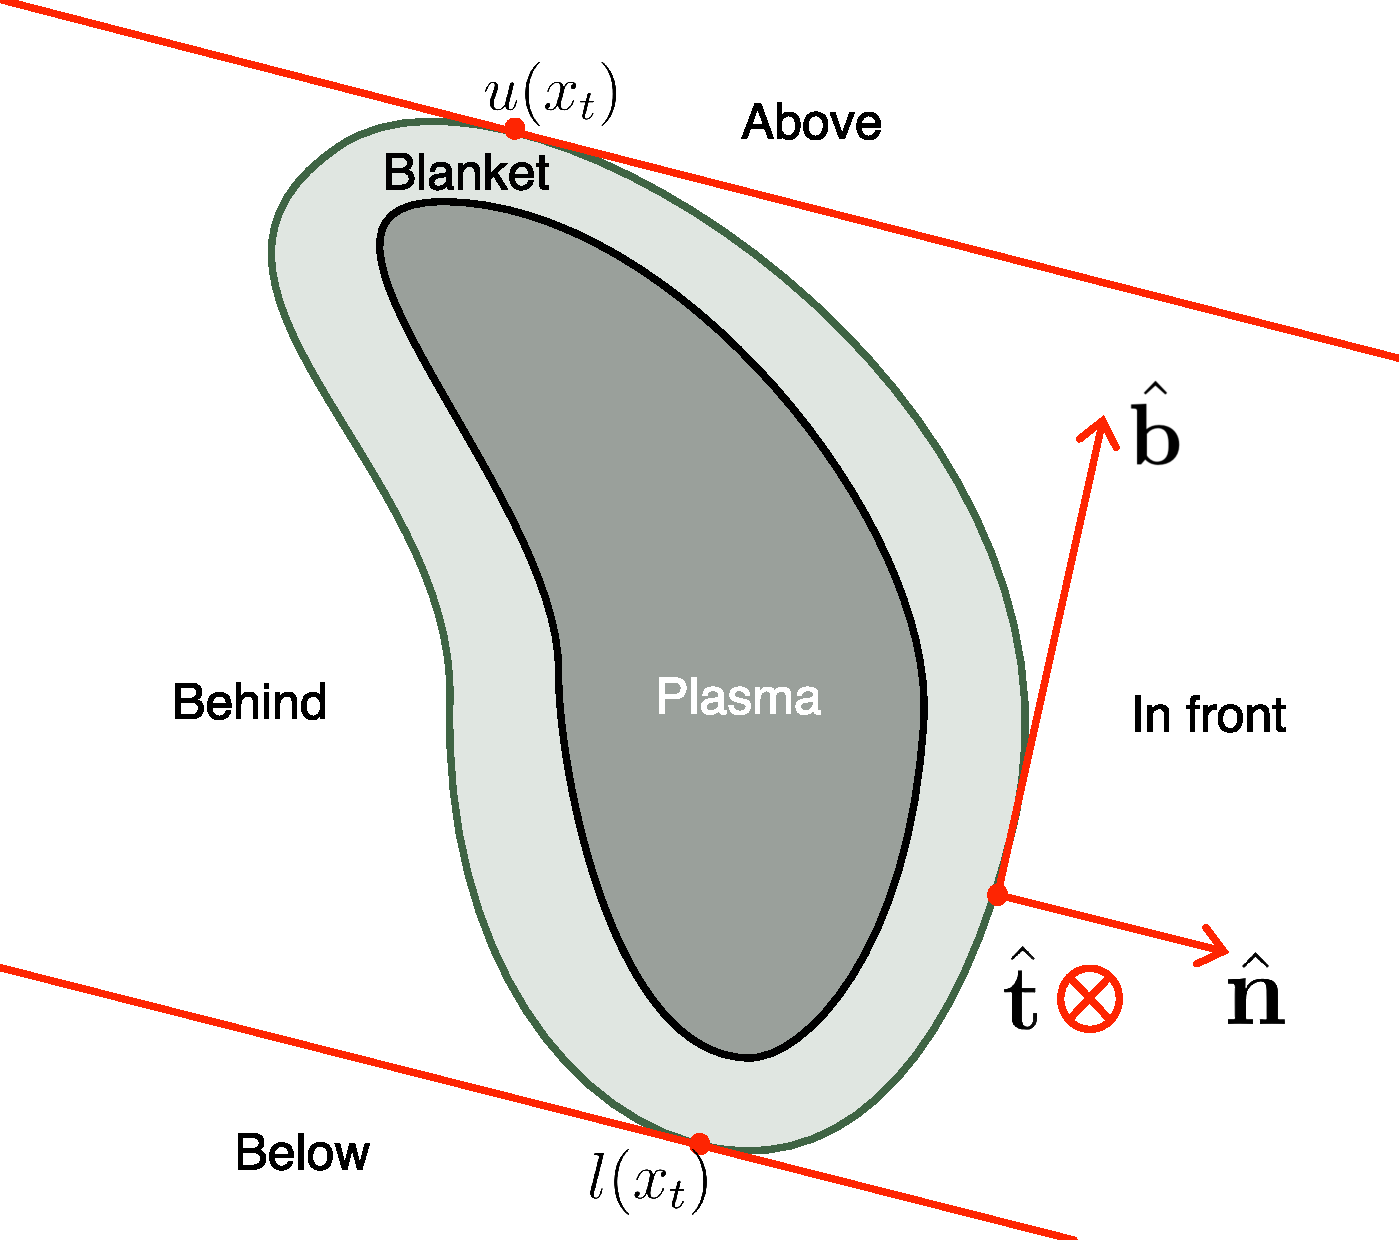
\includegraphics[width=\textwidth]{figures/position_relative_to_vessel.pdf}
    \caption{Sketch of coil elements that are in front, above, behind, or below the vessel.}
    \label{fig.sketch_condition}
\end{figure}
\begin{enumerate}
    \item The point is below the upper envelop, $b^c_i\leq b^u_i$
    \item The point is above the lower envelop, $b^c_i\geq b^l_i$
    \item If $b^c_i>0$, the point needs to be in front of $\mathbf{u}(t^c_i)$, \textit{i.e.} $n^c_i\geq n^u_i$
    \item If $b^c_i<0$, the point needs to be in front of $\mathbf{l}(t^c_i)$, \textit{i.e.} $n^c_i\geq n^l_i$
\end{enumerate}
where we used the notation 
\begin{align}
    b^u_i &= \mathbf{u}(t^c_i)\cdot\hat{\mathbf{b}}\\
    b^l_i &= \mathbf{l}(t^c_i)\cdot\hat{\mathbf{b}}\\
    n^u_i &= \mathbf{u}(t^c_i)\cdot\hat{\mathbf{n}}\\
    n^l_i &= \mathbf{l}(t^c_i)\cdot\hat{\mathbf{n}}.
\end{align}
For each point $\mathbf{x}^c_i$, we then evaluate
\begin{equation}
    \Lambda(\mathbf{x}^c_i,\tilde{\mathbf{x}}) = \mathcal{H}(b^u_i-b^c_i)\mathcal{H}(b^c_i-b^l_i))\left\{\mathcal{H}(-b^c_i)\mathcal{H}(n^c_i-n^l_i)+\mathcal{H}(b^c_i)\mathcal{H}(n^c_i-n^u_i)\right\},\label{eq.test}
\end{equation}
where $\mathcal{H}$ is the Heaviside function, and $\Lambda=1$ if conditions (1)-(4) are satisfied, and $\Lambda=0$ otherwise. Then,
\begin{equation}
    d_i = k\left[\Lambda(\mathbf{x}^c_i,\tilde{\mathbf{x}})-1\right]\sqrt{(b^c_i)^2 + (t^c_i)^2}, 
\end{equation}
where $k$ is a parameter. The metric $d_i$ is then equal to the distance from $\tilde{\mathbf{x}}$ to $\mathbf{x}_p$ in the $(\hat{\mathbf{t}},\hat{\textbf{b}})$-plane if conditions (1)-(4) are satisfied, and is equal to a number of the order of $k$ otherwise. The maximum port size is then given by
\begin{equation}
    r_{port}(\tilde{\mathbf{x}}) = \min\{r_{port}^{lim}, \min_{i\in\{1,\ldots,N_{coils}N_{pts}\}}d_i\}. \label{eq.port_size}
\end{equation}
Finally, the maximum port size on the vessel boundary is obtained by taking the maximum over $(\theta,\phi)$,
\begin{equation}
    r^{max}_{port} = \max_{(\theta,\phi)\in[0,2\pi]\times[0,2\pi/N_f]}r_{port}(\tilde{\mathbf{x}}(\theta,\phi)). \label{eq.max_port_size}
\end{equation}
In practice, we limit the search to regions facing the outboard side of the device, by constraining the poloidal angle to remain within some bounds, $\theta\in[-\pi/2,\pi/2]$.

To allow optimization of the maximum port size, Eq.(\ref{eq.max_port_size}), the metric $r^{max}_{port}$ needs to be differentiable with respect to the coils degrees of freedom, \textit{i.e.} the coils Fourier harmonics. This property is achieved by approximating the maximum and minimum functions in Eq.(\ref{eq.port_size}) by the p-norm,
\begin{equation}
    ||\{f_i\}||_p \approx \left[\sum_i f_i^{p}\right]^{1/p},
\end{equation}
with $\min_i f_i \approx ||\{f_i\}||_p$ for $p\ll-1$ and $\max_i f_i \approx ||\{f_i\}||_p$ for $p\gg1$, and approximating the Heaviside functions in Eq.(\ref{eq.test}) by the logistic function,
\begin{equation}
    \mathcal{H}(x) \approx \frac{1}{2} + \frac{1}{2}\tanh(kx),
\end{equation}
with $k\gg1$. 





\section{Optimiziting stellarator coils for large port size}
\subsection{Stage II optimization}
To optimize the port size of a given configuration, we first start by a standard stage-II optimization. A coil set is sought that accurately reproduce the plasma boundary, \textit{i.e.} where the magnetic field produced by the coils normal to the target plasma boundary is small. This is obtained by minimizing the quadratic flux
\begin{equation}
    \psi_n(\boldsymbol\chi, \mathbf{I}) = \frac{1}{2} \int_{S} (\mathbf{B}\cdot \hat{\mathbf{n}})^2 ds, \label{eq.quadratic_flux}
\end{equation}
where $S$ is the plasma boundary, and here $\mathbf{\hat{n}}$ refers to the surface unit normal vector. The array $\boldsymbol\chi_i$ is an array containing all the curve $\Gamma_i$ degrees of freedom, and $I_i$ is the current in the coil described by $\Gamma_i$. The vector $\boldsymbol{\chi}$ contains the degrees of freedom of all the coils, and the vector $\mathbf{I}$ contains the current from all the coils.  In addition, constraints on the coils length $L_j$, the toroidal flux $\psi_t$, the coil-to-coil distance $d_{cc}$ and the coil-to-plasma distance $d_{cs}$ are enforced, with
\begin{align}
    L_i(\boldsymbol\chi_i) &= \max\left(\int_{\Gamma_i} dl - L_0, 0\right)^2\\
    P_{\psi_t}(\boldsymbol\chi, \mathbf{I}) &= \left(\int_{S_{\varphi}} \mathbf{B}(\boldsymbol\chi, \mathbf{I}) \cdot \mathbf{n} ~ds - \psi_{t,0}\right)^2\\
    d_{cc}(\boldsymbol\chi) &= \sum_{i=1}^{N_{coils}} \sum_{j = 1}^{i-1} \int_{\Gamma_i} \int_{\Gamma_j} \max(d_{cc,0} - \| \mathbf{r}_i - \mathbf{r}_j \|_2, 0)^2 ~dl_j ~dl_i\\
    d_{cs}(\boldsymbol\chi) &= \sum_{i = 1}^{N_{coils}} \int_{\Gamma_i} \int_S \max(d_{cs,0} - \| \mathbf{r}_i - \mathbf{s} \|_2, 0)^2 ~dl_i ~ds
\end{align}
where The scalar $L_0$ is the maximum length for a coil, $\psi_{t,0}$ is the target toroidal magnetic flux, $d_{cc,0}$ is the maximum coil-to-coil distance, and $d_{cs,0}$ is the maximum coil-to-surface distance. The full objective function is then
\begin{equation}
    f_1(\boldsymbol\chi,\mathbf{I}) = \psi_n + w_l\sum_{i=1}^{N_{coils}}L_i + w_tP_{\psi_t} + w_{cc}d_{cc} + w_{cs}d_{cs},
\end{equation}
where $(w_l,w_t,w_{cc},w_{cs})$ are user-supplied weights, and the dependence on $\boldsymbol{\chi}$ and $\mathbf{I}$ have been dropped on the right-hand-side. There are no ways to know what choice of weights will lead to the best results \textit{a priori} --- instead, in all results presented in this paper, we scanned various combination of weights until finding satisfactory results. We use the simsopt python framework for stellarator optimization \cite{landreman_2021} to drive the optimization

\subsection{Port size optimization}
After completing the stage II optimization, we maximize the port size defined in Eq.(\ref{eq.max_port_size}) while keeping the quadratic flux (\ref{eq.quadratic_flux}) below a threshold $\psi_{n,0}$. To do so, we define the penalty
\begin{equation}
    P_{\psi_n}(\boldsymbol\chi, \mathbf{I}) = \max(\psi_n-\psi_{n,0}, 0 )^2,
\end{equation}
and we minimize
\begin{equation}
    f_2(\boldsymbol\chi, \mathbf{I}) = -r^{max}_{port} + w_nP_{\psi_n} + w_l\sum_{i=1}^{N_{coils}}L_i + w_tP_{\psi_t} + w_{cc}d_{cc} + w_{cs}d_{cs},
\end{equation}
where $w_n$ is a user-supplied weight, and the dependence on $\boldsymbol{\chi}$ and $\mathbf{I}$ have been dropped. Again, we scan various value for the weight $w_n$ until satisfactory results are obtained. Finally, the metric (\ref{eq.max_port_size}) is implemented usind the JAX python library for automatic differentiation \cite{jax2018github}, providing derivatives of $r^{max}_{port}$ with respect to the coils degrees of freedom at a fraction of the computational needed to evaluate the derivatives of $r^{max}_{port}$ using finite differences. 







\newpage
\section*{Acknowledgements}
\begin{itemize}
\item L. Jorrit, M. Zarnstoff, J. Schwartz, M. Churchill useful discussion
\end{itemize}







\printbibliography

\end{document}

